\section{Hardware Framework}
\label{sec:hardwareframework}

\subsection{Purpose}
The hardware framework allows different chips to be utilized with the same 
\emphasize{Intermediate Language} code generated from our 
software package ``PLCEdit''.
The hardware must meet the minimum requirements defined by Section \ref{sec:hardwareplatform}. 
The framework consists of a bunch of definitions which map the symbolic software 
references to hardware specific calls. In addition the framework is also 
responsible for properly initializing the chip and performing any clean 
up operations once the chip completes execution.


\subsection{Hardware Framework Overview}

\begin{figure}[htp]
    \centering
    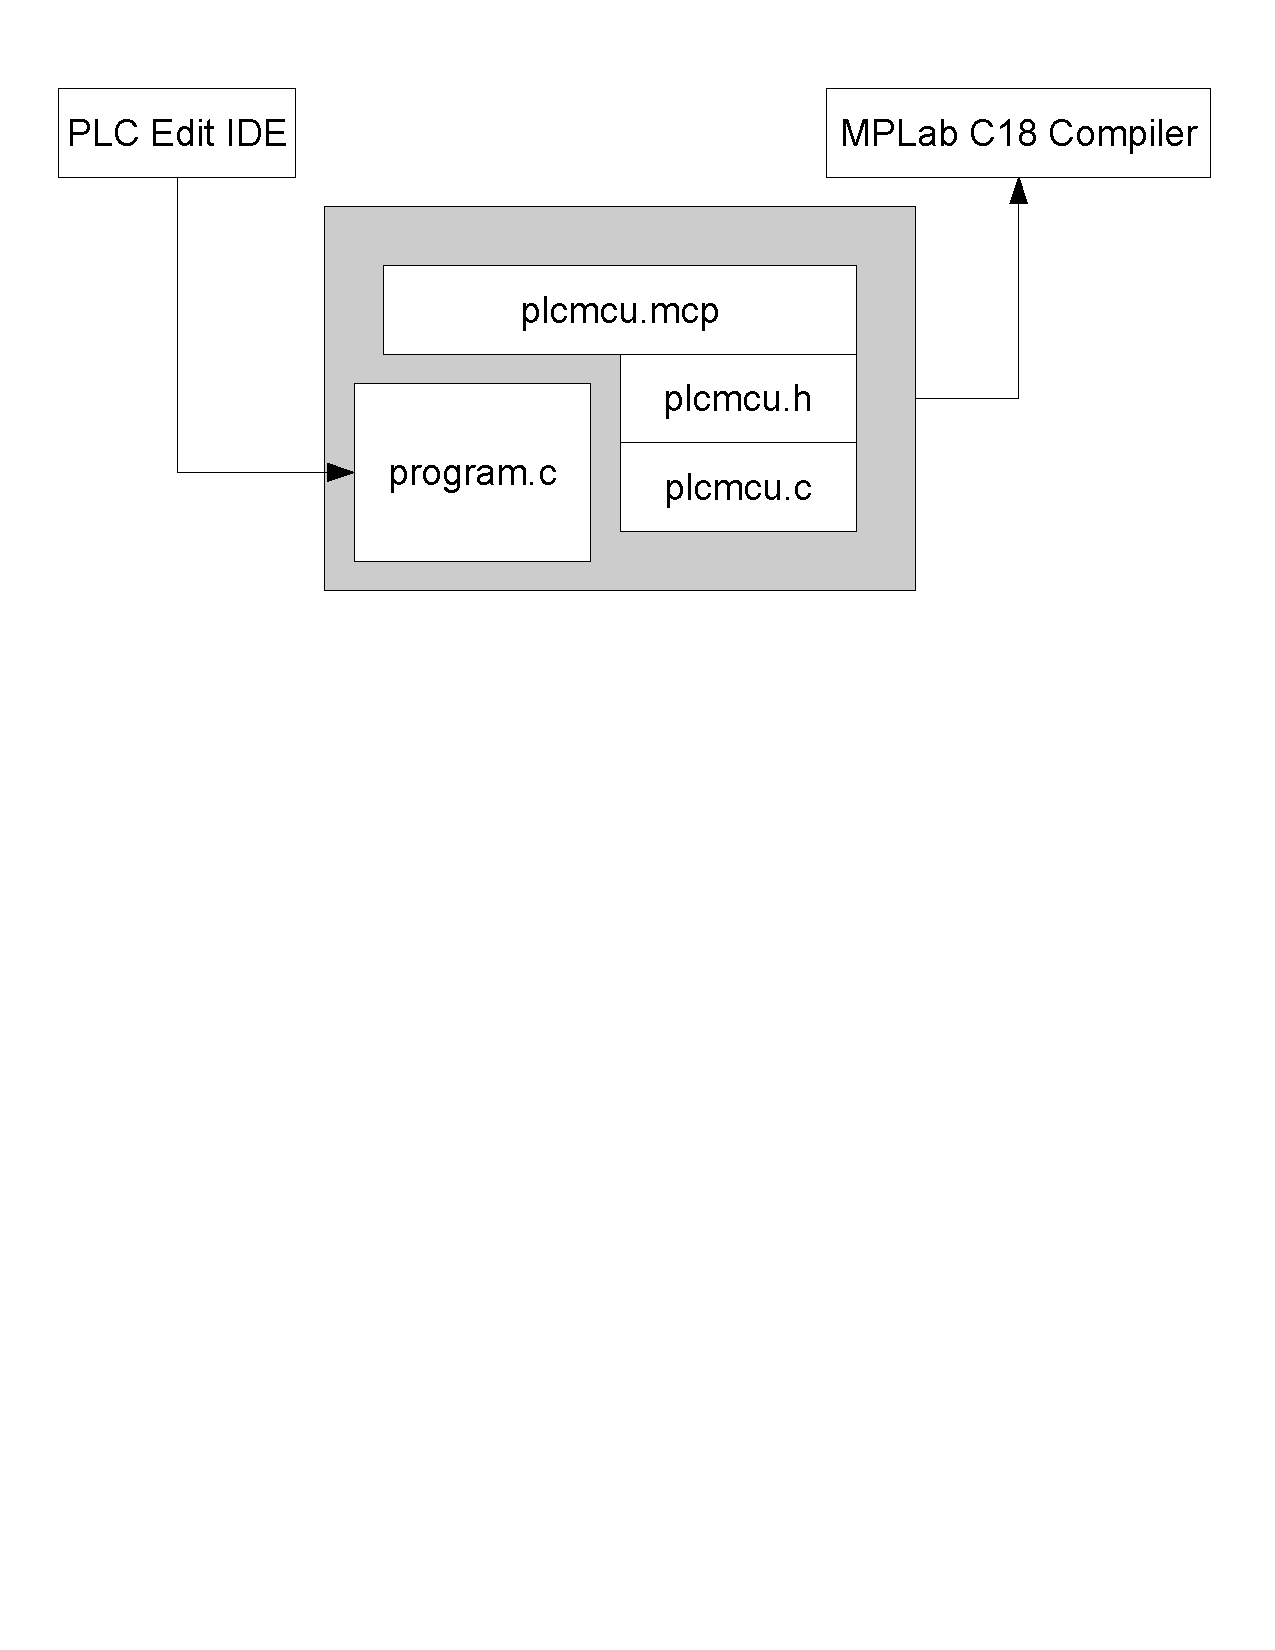
\includegraphics[trim= 10mm 150mm 10mm 10mm, clip, width=\imgmedium]{./images/hardwareframework.pdf}
    \caption{Hardware Framework Components}
    \label{fig:hardwareframework}
\end{figure}

The hardware framework was designed to allow multiple targets. Our IDE generates 
a program.c file that refers to hardware functions and definitions implemented 
in ``plcmcu.h'' and ``plcmcu.c'' to be combined with an optional ``plcmcu.mcp'' 
project file. ``plcmcu.h'' contains definitions of the hardware. These are usually designer choices such as oscillator selection, and which ports on the chip they will be using for input and output. ``plcmcu.c'' will implement any function calls that are required and take care of any chip initializations. In addition it is ``plcmcu.c'' job to call the user generated ``program.c'' once the chip is fully initialized and setup. The entire framework is then sent to the MPLab C18 compiler, or a compiler of the implementer's choosing. In the next section we will show and comment on some of the sample code for our prototype system.


\subsection{Sub-Component Implementations} 

\noindent\textbf{File:} plcmcu.h

\noindent\textbf{Section:} Chip configuration 

\noindent\textbf{Description:} Sets configuration bits for the chip that cannot be done at run time.

\noindent\textbf{Code:}



\begin{lstlisting}[frame=single]
...
#pragma config OSC = HSPLL //set occilator to HS-PLL
#pragma config OSCS = OFF //disable occilator switch
#pragma config PWRT = OFF //enable power on timer
#pragma config WDT = OFF //disable watchdog timer
#pragma config LVP = OFF //disable low power programming
...
\end{lstlisting}



\noindent\textbf{File:} plcmcu.c

\noindent\textbf{Routine:} init\_chip(void)

\noindent\textbf{Description:} Initializes any chip specific configuration bits that must be done at run time.

\noindent\textbf{Code:}



\begin{lstlisting}[frame=single]
...
void init_chip(void)
{	
	TRISA = 0xFF; //set all portA to input
	TRISB = 0x00; //set all portB to output
}
...
\end{lstlisting}



\subsection{Hardware Specific Definitions}

Hardware specific definitions are reserved for mapping specific characteristics 
of the hardware to match up with the references in the \emphasize{Intermediate Language}. 
For example it may be necessary to define the input and output ports to a specific port on the chip itself.



\begin{lstlisting}[frame=single]
...
/* PORT specification */
#define PORTOUT PORTB
#define PORTIN PORTA
...
\end{lstlisting}



\subsection{Hardware Specific Implementations}

Function calls from our software that access more complex operations 
may be required to be implemented directly into hardware. Our current 
software only requires that the routine for delaying the execution by a 
number of milliseconds is implemented. It is done as follows (please 
note for layout reasons we are using underscore when code should be 
on the same line):

\textbf{File:}plcmcu.h



\begin{lstlisting}[frame=single]
/* CLOCK specification */
...

#define OCCILATOR 10000000 
//our occilator in seconds
#define TCYTIME 1 
//now many cycles / instruction 4 for non PLL 1 for PLL 

#define TCYTICK OCCILATOR / TCYTIME 
//how long per instruction tick
#define MSTIME 1000 
//milliseconds to seconds

#define MSTCY TCYTICK / MSTIME 
//how many clocks in a ms (10000 for pll)

//crystal select block
#if (MSTCY >= 10000)
	#define DEFDELAY(timevalms) _
	Delay10KTCYx(timevalms * (char) (MSTCY/10000))
#endif
#if (MSTCY >= 1000 && MSTCY void delayms(int time)
{
	DEFDELAY(time);
}< 10000)
	#define DEFDELAY(timevalms) _ 
	Delay1KTCYx(timevalms * (char) (MSTCY/1000))
#endif
#if (MSTCY < 1000)
	#error "Unsupported OCCILATOR defined by hardware" _ 
	" manufacturer please ensure crystal is faster than 1Mhz"
#endif

/* End CLOCK specification */

...
\end{lstlisting}



\textbf{File:} plcmcu.c



\begin{lstlisting}[frame=single]
...
void delayms(int time)
{
	DEFDELAY(time);
}
...
\end{lstlisting}



It is highly recommended to avoid macros where possible however the nature of 
the PIC18F452 required macros in order to prevent inaccurate delays caused by 
repeatedly calculating the oscillator conversions at run time.